\begin{section}{Resultados}

A continuaci\'on, algunos resultados interesantes.

\begin{subsection}{Caso I}

Input: (AVIONES/BARCOS)

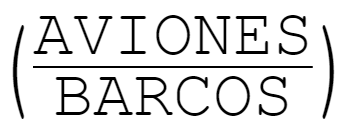
\includegraphics[scale=0.5]{./imgs/aviones.png}

La dificultad de este caso recae la divisi\'on de dos nodos no terminales (concatenaciones), donde la barra debe ajustarse al tama\~no del mayor de ellos y se debe centrar al menor. As\'i mismo, se deben ajustar los par\'entensis para abarcar toda la divisi\'on. 

\end{subsection}

\begin{subsection}{Caso II}

Input: MAR/(AGUA+SAL)

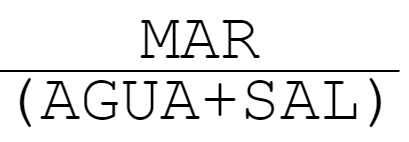
\includegraphics[scale=0.5]{./imgs/mar.png}

En esta oportunidad, la divisi\'on de, nuevamente, dos nodos no terminales (concatenaciones), con la diferencia de que los par\'entensis solo abarcan al denominador de la misma. Adem\'as, en este caso el numerador es aquel de longitud menor y por ende el que debe ser centrado.

\end{subsection}
\begin{subsection}{Caso III}

Input: VIENTO\^{}\{FUERTE\}/VELERO\_\{EN+PROBLEMAS\}

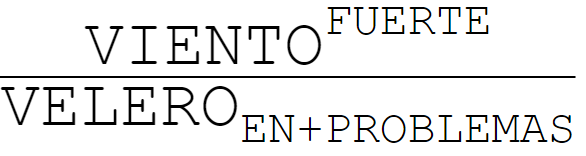
\includegraphics[scale=0.5]{./imgs/velero.png}

En este caso se incluyen sub\'indices y super\'indices, dentro de una divisi\'on, que es el nodo problem\'atico por excelencia.

\end{subsection}
\begin{subsection}{Caso IV}

Input: SUPER\^{}\{HEROE\}\_\{VILLANO\}


\includegraphics[scale=0.5]{./imgs/super.png}

Por \'ultimo, la combinaci\'on de sub y super\'indices, ambos como concatenaciones encerradas por llaves para agruparlas.

\end{subsection}
\end{section}
